\documentclass[11pt]{article}
\usepackage{amsmath, amssymb, amsfonts,  graphicx, enumerate, float, wrapfig}
\usepackage[margin=0.5in]{geometry}
\graphicspath{{./}}
\newcommand*{\vs}{\vspace{1cm}}
\newcommand*{\next}{\noindent}
\newcommand*{\set}{\setcounter{equation}{0}}


\title{3.3 Increasing and Decreasing Functions and the First Derivative Test}
\author{Juan J. Moreno Santos}
\date{October 2023}

\begin{document}
\maketitle

\section{Use the graph of $f$ to find (a) the largest open interval on which $f$ is increasing, and (b) the largest open interval on which $f$ is decreasing.}
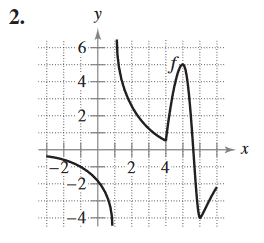
\includegraphics{2.png}
\begin{enumerate}[(a)]
    \item The intervals in which $f$ is increasing are (4,5) and (6, 7). They are also the largest.
    \item The intervals in which $f$ is decreasing are (-3, 1), (1, 4), and (5, 6). (-3, 1) is the largest.
\end{enumerate}

\section{Use the graph to estimate the open intervals on which the function is increasing or decreasing. Then find the open intervals analytically.}
4.\[y=-(x+1)^2\]
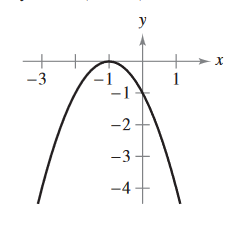
\includegraphics{4.png}\\
Graphically, $f$ increases on 
$(-\infty, -1)$ and decreases on $(-1, \infty)$.\\
Analytically, $y'=-2(x+1)\therefore x=-1$ is a critical number.\\

\begin{flushleft}
    \begin{table}
        \begin{tabular}{|l|l|l|} % Alignment: l- left, r- right, c- center. Pipes | separate columns
        \hline
        $\text{Test intervals}$ & $-\infty<x<-1$ & $-1<x<\infty$\\ \hline
        $y'\,\,\,\,\text{sign}$ & $y'>0$ & $y'<0$ \\ \hline
        $\text{Conclusion}$ & Increasing & Decreasing\\
        \hline
        \end{tabular}
    \end{table}
\end{flushleft}

\next
8.\[y=\frac{x^2}{2x-1}\]\\
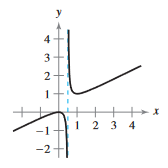
\includegraphics{8.png}\\
Graphically, y increases on $(-\infty, 0)$ and $(1, \infty)$, and decreases on $(0, \frac{1}{2})$ and $(\frac{1}{2}, 1)$.\\
Analytically, $y'=\frac{(2x-1)2x-x^2(2)}{(2x-1)^2}=\frac{2x^2-2x}{(2x-1)^2}=\frac{2x(x-1)}{(2x-1)^2}\therefore x=0, 1$ are critical numbers, and there is a discontinuity at $x=\frac{1}{2}$.
\begin{flushleft}
    \begin{table}[h]
        \begin{tabular}{|l|l|l|l|l|} % Alignment: l- left, r- right, c- center. Pipes | separate columns
        \hline
        $\text{Test intervals}$ & $-\infty<x<0$ & $0<x<\frac{1}{2}$ & $\frac{1}{2}<x<1$ & $1<x<\infty$\\ \hline
        $y'\,\,\,\,\text{sign}$ & $y'>0$ & $y'<0$ & $y'<0$ & $y'>0$\\ \hline
        $\text{Conclusion}$ & Increasing & Decreasing & Decreasing & Increasing\\
        \hline
        \end{tabular}
    \end{table}
\end{flushleft}

\section{Identify the open intervals on which the function is increasing or decreasing.}
10.\begin{align}
    h(x)&=27x-x^3\\
    h'(x)&=27-3x^2\\
    &=3(3-x)(3+x)\\
    &=0
\end{align}
$x=\pm 3$ are critical numbers.

\begin{flushleft}
    \begin{table}[h]
        \begin{tabular}{|l|l|l|l|} % Alignment: l- left, r- right, c- center. Pipes | separate columns
        \hline
        $\text{Test intervals}$ & $-\infty<x<-3$ & $-3<x<3$ & $3<x<\infty$\\ \hline
        $h'\,\,\,\,\text{sign}$ & $h'<0$ & $h'>0$ & $h'<0$\\ \hline
        $\text{Conclusion}$ & Decreasing & Increasing & Decreasing\\
        \hline
        \end{tabular}
    \end{table}
\end{flushleft}

The function is increasing on (-3, 3) and decreasing on $(-\infty, -3)$ and $(3, \infty)$.

\vs
\next
14.\begin{align}
    h(x)&=\cos\frac{x}{2},\,\,\,\,0<x<2\pi\\
    h'(x)&=-\frac{1}{2}\sin\frac{x}{2}
\end{align}
The function has no critical numbers.
\begin{flushleft}
    \begin{table}[h]
        \begin{tabular}{|l|l|} % Alignment: l- left, r- right, c- center. Pipes | separate columns
        \hline
        $\text{Test intervals}$ & $0<x<2\pi$\\ \hline
        $h'\,\,\,\,\text{sign}$ & $h'<0$\\ \hline
        $\text{Conclusion}$ & Decreasing\\
        \hline
        \end{tabular}
    \end{table}
\end{flushleft}
The function is decreasing on $0<x<2\pi$.

\section{(a) Find the critical numbers fof $f$ (if any), (b) find the open interval(s) on which the function is increasing or decreasing, (c) apply the First Derivative Test to identify all relative extrema.}
18.\begin{enumerate}[(a)]
    \item \begin{align}
        \set
        f(x)=&x^2+6x+10\\
        f'(x)&=2x+6
    \end{align}\\
    $x=-3$ is a critical number.
    \begin{flushleft}
        \begin{table}[h]
                \begin{tabular}{|l|l|l|} % Alignment: l- left, r- right, c- center. Pipes | separate columns
                    \hline
                    $\text{Test intervals}$ & $-\infty<x<-3$ & $-3<x<\infty$\\ \hline
                    $f'\,\,\,\,\text{sign}$ & $f'<0$ & $f'>0$\\ \hline
                    $\text{Conclusion}$ & Decreasing & Increasing\\
                    \hline
             \end{tabular}
            \end{table}
        \end{flushleft}
        \item The function is decreasing on $(-\infty, -3)$ and increasing on $(3, \infty)$\\
        \item (-3, 1) is the relative minimum.
\end{enumerate}

\vs
\next
22.\begin{enumerate}[(a)]
    \item \begin{align}
        \set
        f(x)&=x^3-6x^2+15\\
        f'(x)&=3x^2-12x\\
        &=3x(x-4)
    \end{align}\\
    $x=0, 4$ are critical numbers.
    \newpage
    \begin{flushleft}
        \begin{table}
                \begin{tabular}{|l|l|l|l|} % Alignment: l- left, r- right, c- center. Pipes | separate columns
                    \hline
                    $\text{Test intervals}$ & $-\infty<x<0$ & $0<x<4$ & $4<x<\infty$\\ \hline
                    $f'\,\,\,\,\text{sign}$ & $f'>0$ & $f'<0$ & $f'>0$\\ \hline
                    $\text{Conclusion}$ & Increasing & Decreasing & Increasing\\
                    \hline
             \end{tabular}
            \end{table}
        \end{flushleft}
        \item The function is decreasing on $(0, 4)$ and increasing on $(-\infty, 0)$ and $(4, \infty)$.\\
        \item (4, -17) is the relative minimum and (0, 15) the relative maximum.
\end{enumerate}

\vs
\next
26.\begin{enumerate}[(a)]
    \item \begin{align}
        \set
        f(x)&=x^4-32x+4\\
        f'(x)&=4x^3-32\\
        &=4(x^3-8)
    \end{align}\\
    $x=2$ is a critical number.
    \begin{flushleft}
        \begin{table}[h]
                \begin{tabular}{|l|l|l|} % Alignment: l- left, r- right, c- center. Pipes | separate columns
                    \hline
                    $\text{Test intervals}$ & $-\infty<x<2$ & $2<x<\infty$\\ \hline
                    $f'\,\,\,\,\text{sign}$ & $f'<0$ & $f'>0$\\ \hline
                    $\text{Conclusion}$ & Decreasing & Increasing\\
                    \hline
             \end{tabular}
            \end{table}
        \end{flushleft}
        \item The function is decreasing on $(-\infty, 2)$ and increasing on $(2, \infty)$\\
        \item (2, -44) is the relative minimum.
\end{enumerate}

\vs
\next
30.\begin{enumerate}[(a)]
    \item \begin{align}
        \set
        f(x)&=(x-3)^{1/3}\\
        f'(x)&=\frac{1}{3}(x-3)^{-2/3}\\
        &=\frac{1}{3(x-3)^2/3}
    \end{align}\\
    $x=3$ is a critical number.
    \begin{flushleft}
        \begin{table}[h]
                \begin{tabular}{|l|l|l|} % Alignment: l- left, r- right, c- center. Pipes | separate columns
                    \hline
                    $\text{Test intervals}$ & $-\infty<x<3$ & $3<x<\infty$\\ \hline
                    $f'\,\,\,\,\text{sign}$ & $f'>0$ & $f'>0$\\ \hline
                    $\text{Conclusion}$ & Increasing & Increasing\\
                    \hline
             \end{tabular}
            \end{table}
        \end{flushleft}
        \item The function is increasing on $(-\infty, \infty)$
        \item The function has no relative extrema.
\end{enumerate}

\vs
\next
34.\begin{enumerate}[(a)]
    \item \begin{align}
        \set
        f(x)&=\frac{x}{x+3}\\
        f'(x)&=\frac{(x+3)-x}{(x+3)^2}\\
        &=\frac{3}{(x+3)^2}
    \end{align}\\
    The function has no critical numbers but a discontinuity at $x=-3$.
    \begin{flushleft}
        \begin{table}[h]
                \begin{tabular}{|l|l|l|}
                    \hline
                    $\text{Test intervals}$ & $-\infty<x<-3$ & $-3<x<\infty$\\ \hline
                    $f'\,\,\,\,\text{sign}$ & $f'>0$ & $f'>0$\\ \hline
                    $\text{Conclusion}$ & Increasing & Increasing\\
                    \hline
             \end{tabular}
            \end{table}
        \end{flushleft}
        \item The function is increasing on $(-\infty, -3)$ and $(-3, \infty)$.
        \item The function has no relative extrema.
\end{enumerate}

\vs
\next
38.\begin{enumerate}[(a)]
    \item \begin{align}
        \set
        f(x)&=\frac{x^2-3x-4}{x-3}\\
        f'(x)&=\frac{(2x-3)(x-2)-(x^2-3x-4)}{(x-2)^2}\\
        &=\frac{x^2-4x+10}{(x-2)^2}
    \end{align}\\
    The function has a discontinuity at $x=2$.
    \begin{flushleft}
        \begin{table}[h]
                \begin{tabular}{|l|l|l|}
                    \hline
                    $\text{Test intervals}$ & $-\infty<x<2$ & $2<x<\infty$\\ \hline
                    $f'\,\,\,\,\text{sign}$ & $f'>0$ & $f'>0$\\ \hline
                    $\text{Conclusion}$ & Increasing & Increasing\\
                    \hline
             \end{tabular}
            \end{table}
        \end{flushleft}
        \item The function is increasing on $(-\infty, 2)$ and $(2, \infty)$.
        \item The function has no relative extrema.
\end{enumerate}

\vs
\next
42.\begin{enumerate}[(a)]
    \item \begin{align}
        \set
        f(x)&=\begin{cases}
            -x^3+1,\,\,\,\, x\leq 0\\
            -x^2+2x,\,\,\, x>0
        \end{cases}\\
        f'(x)&=\begin{cases}
            -3x^2,\,\,\,\, x<0\\
            -3x+2,\,\,\,\ x>0\\
        \end{cases}
    \end{align}\\
    $x=0, 1$ are critical numbers.
    \begin{flushleft}
        \begin{table}[h]
                \begin{tabular}{|l|l|l|l|}
                    \hline
                    $\text{Test intervals}$ & $-\infty<x<0$ & $0<x<1$ & $1<x<\infty$\\ \hline
                    $f'\,\,\,\,\text{sign}$ & $f'<0$ & $f'>0$ & $f'<0$\\ \hline
                    $\text{Conclusion}$ & Decreasing & Increasing & Decreasing\\
                    \hline
             \end{tabular}
            \end{table}
        \end{flushleft}
        \item The function is increasing on $0, 1)$ and decreasing on $(-\infty, 0)$ and $(1, \infty)$
        \item (1, 1) is a relative maximum.
\end{enumerate}

\section{Consider the function on the interval $(0, 2\pi)$. For each function, (a) find the open interval(s) in which the function is increasding or decreasing, and (b) apply the First Derivative Test to identify all relative extrema.}
44.\begin{enumerate}[(a)]
    \item \begin{align}
        \set
        f(x)&=\sin x \cos x+5\\
        &=\frac{1}{2}\sin 2x+5,\,\,\,\,0<x<2\pi\\
        f'(x)&=\cos 2x
    \end{align}\\
    $x=\frac{\pi}{4}, \frac{3\pi}{4}, \frac{5\pi}{4}, \frac{7\pi}{4}$ are critical numbers.
    \begin{flushleft}
        \begin{table}[h]
                \begin{tabular}{|l|l|l|l|l|l|}
                    \hline
                    $\text{Test intervals}$ & $0<x<\frac{\pi}{4}$ & $\frac{\pi}{4}<x<\frac{3\pi}{4}$ & $\frac{3\pi}{4}<x<\frac{5\pi}{4}$ & $\frac{5\pi}{4}<x<\frac{7\pi}{4}$ & $\frac{7\pi}{4}<x<2\pi$\\ \hline
                    $f'\,\,\,\,\text{sign}$ & $f'>0$ & $f'<0$ & $f'>0$ & $f'<0$ & $f'>0$\\ \hline
                    $\text{Conclusion}$ & Increasing & Decreasing & Increasing & Decreasing & Increasing\\
                    \hline
             \end{tabular}
            \end{table}
        \end{flushleft}
        The function is increasing on $\left(0, \frac{\pi}{4}\right)$, $\left(\frac{3\pi}{4}, \frac{5\pi}{4}\right)$ and $\left(\frac{7\pi}{4}, 2\pi\right)$, and decreasing on $\left(\frac{\pi}{4}, \frac{3\pi}{4}\right)$ and $\left(\frac{5\pi}{4}, \frac{7\pi}{4}\right)$.
        \item $\left(\frac{\pi}{4}, \frac{11}{2}\right)$ and $\left(\frac{5\pi}{4}, \frac{11}{2}\right)$ are the relative maxima, and $\left(\frac{3\pi}{4}, \frac{9}{2}\right)$ and $\left(\frac{7\pi}{4}, \frac{9}{2}\right)$ the relative minima.
\end{enumerate}

48.\begin{enumerate}[(a)]
    \item \begin{align}
        \set
        f(x)&=\sqrt[]{3}\sin x+\cos x\\
        f'(x)&=\sqrt[]{3}\cos x-\sin x=0\\
        \tan x&=\sqrt[]{3}
    \end{align}\\
    $x=\frac{\pi}{3}, \frac{4\pi}{3}$ are critical numbers.
    \begin{flushleft}
        \begin{table}[h]
                \begin{tabular}{|l|l|l|l|}
                    \hline
                    $\text{Test intervals}$ & $0<x<\frac{\pi}{3}$ & $\frac{\pi}{3}<\frac{4\pi}{3}$ & $\frac{4\pi}{3}<x<2\pi$\\ \hline
                    $f'\,\,\,\,\text{sign}$ & $f'>0$ & $f'<0$ & $f'<0$\\ \hline
                    $\text{Conclusion}$ & Increasing & Decreasing & Decreasing\\
                    \hline
             \end{tabular}
            \end{table}
        \end{flushleft}
        The function is increasing on $\left(0, \frac{\pi}{3}\right) \text{and} \left(\frac{4\pi}{3}, 2\pi\right)$, and decreasing on $\left(\frac{\pi}{3}, \frac{4\pi}{3}\right)$
        \item $\left(\frac{\pi}{3}, 2\right)$ is the relative maximum, and $\left(\frac{4\pi}{3}, -2\right)$ the relative minimum.
\end{enumerate}

\section{Use symmetry, extrema, and zeros to sketch the graph of $f$. How do the functions $f$ and $g$ differ?}
58.\[f(t)=\cos^2t-\sin^2t,\,\,\,\,\, g(t)=1-2\sin^2t\]
\[f(t)=\cos^2t-\sin^2t=1-2\sin^2 t=g(t)\]
\[f'(t)=-4\sin t\cos t=-2\sin 2t\]
$f$ is symmetric to the y-axis and has zeros at $\pm \frac{\pi}{4}$
(0, 1) is the relative maximum, and $\left(-\frac{\pi}{2}, -1\right)$ and $\left(\frac{\pi}{2}, -1\right)$ are the relative minima.\\
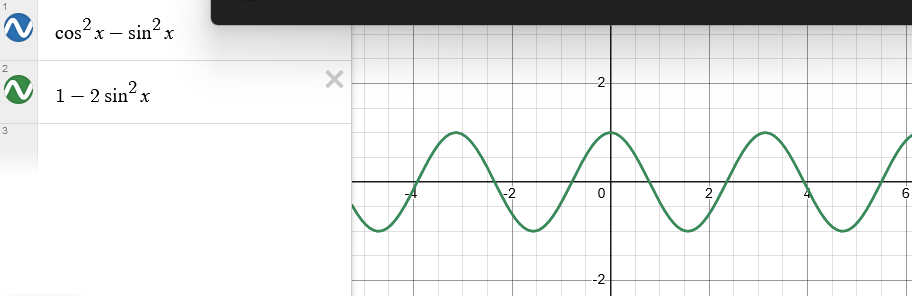
\includegraphics{58.png}\\
$f(x)$ and $g(x)$ are the same graph.

\section{The graph of $f$ is shown. Sketch a graph of the derivative of $f$.}
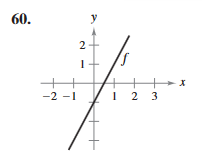
\includegraphics{60a.png}
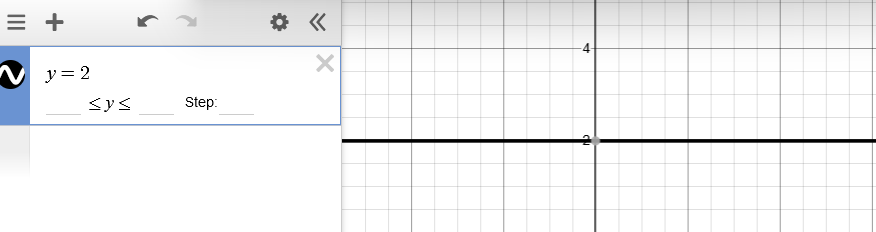
\includegraphics[scale=0.5]{60b.png}\\
\[f'(x)=2\]\\

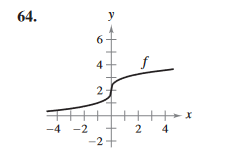
\includegraphics{64.png}
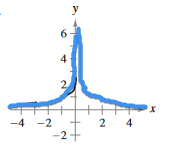
\includegraphics{64b.png}

\section{Use the graph of $f'$ to (a) identify the interval(s) on which $f$ is increasing or decreasing, and (b) estimate the value(s) of $x$ at which $f$ has a relative maximum or minimum.}
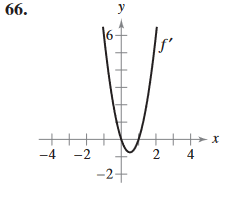
\includegraphics{66.png}
\begin{enumerate}[(a)]
    \item $f$ is increasing on $(-\infty, 0)$ and $(1, \infty)$, and decreasing on (0, 1).
    \item $f$ has a relative maximum and minimum and $x=0$ and $x=1$ respectively.
\end{enumerate}

\section{Use the graph of $f'$ to (a) identify the critical numbers of $f$, and (b) determine whether $f$ has a relative maximum, a relative minimum, or neither at each critical number.}
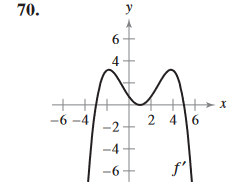
\includegraphics{70.png}
\begin{enumerate}[(a)]
    \item $f'=0$ at $x=-3, 1, 5$
    \item \begin{enumerate}[i.]
        \item $x=-3$ is a relative minimum.
        \item $x=5$ is a relative maximum. 
        \item $x=1$ is neither. 
    \end{enumerate}
\end{enumerate}

\section{The function $f$ is differentiable on the indicated interval. The table shows $f'(x)$ for selected values of $x$. (a) Sketch the graph of $f$, (b) approximate the critical numbers, and (c) identify the relative extrema.}
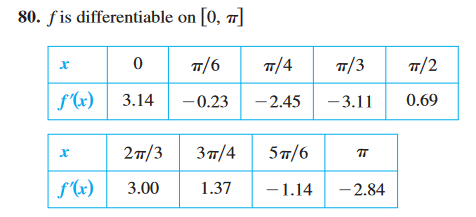
\includegraphics{80a.png}
\begin{enumerate}[(b)]
    \item The critical numbers are in the intervals $\left(0, \frac{\pi}{6}\right)$, $\left(\frac{\pi}{3}, \frac{\pi}{2}\right)$, and $\left(\frac{3\pi}{4}, \frac{5\pi}{6}\right)$.\\
        $f$ is increasing on $\left(0, \frac{\pi}{7}\right)$ and $\left(\frac{3\pi}{7}, \frac{6\pi}{7}\right)$, and decreasing on $\left(\frac{\pi}{7}, \frac{3\pi}{7}\right)$ and $\left(\frac{6\pi}{7}, \pi\right)$.
    \item[(c)] Relative minima occur when $x=\frac{3\pi}{7}, \pi$ and relative maxima occur when $x=\frac{\pi}{7}, \frac{6\pi}{7}$.
\end{enumerate}

\section{Word problems}
82. The concentration $C$ of a chemical in the bloodstream $t$ hours after the injection into muscle tissue is \[C(t)=\frac{3t}{27+t^3},\,\,\,\, t\geq 0\]\\
(a) Complete the table and use it to approximate the time when the concentration is greatest.
\begin{flushleft}
    \begin{table}[h]
            \begin{tabular}{|l|l|l|l|l|l|l|l|}
                \hline
                $t$ & $0$ & $0.5$ & $1$ & $1.5$ & $2$ & $2.5$ & $3$\\ \hline
                $C(t)$ & $0$ & $0.055$ & $0.107$ & $0.148$ & $0.171$ & $0.176$ & $0.167$\\ \hline
         \end{tabular}
    \end{table}
\end{flushleft}
The concentration is greatest at $t=2.5$ hours.\\

\next
(b) Use a graphing utility to graph the concentration function and use the graph to approximate the time when the concentration is the greatest.\\
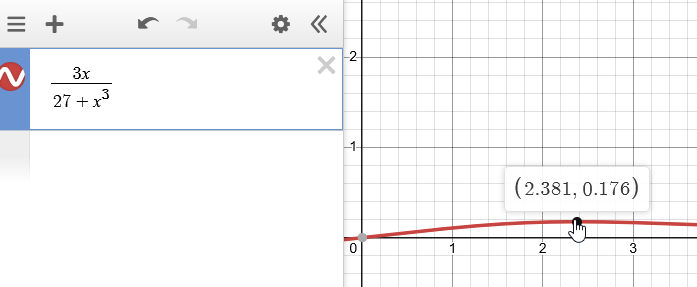
\includegraphics[scale=0.5]{82.png}\\
The concentration is greatest at $t\approx 2.381$ hours.\\

\next
(c) Use calculus to determine analytically the time when the concentration is the greatest.
\begin{align}
    \set
    C'&=\frac{(3)(27+t^3)-(3t)(3t^2)}{(27+t^3)^2}\\
    &=\frac{3(27-2t^3)}{(27+t^3)^2}\\
    &=0\,\,\text{when}\,\, t=\frac{3}{\sqrt[3]{2}}\approx 2.381\,\,\text{hours}
\end{align}
This is a maximum according to the First Derivative Test.

\vs
\next
88. The end-of-year assets of the Medicare Hospital Insurance Trust Fund (in billions of dollars) for the years 1995 through 2006 are shown.\\
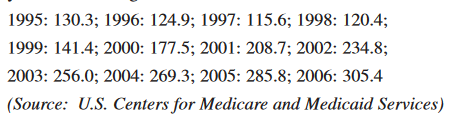
\includegraphics{88.png}\\
(a) Use the regression capabilities of a graphing utility to find a model of the form $M=at^4+bt^3+ct^2+dt+e$ for the data (Let $t=5$ represent 1995.).
\[M=0.03723t^4-1.993t^3+37.986t^2-282.74t+825.7\]\\
(c) Find the minimum value of the model and compare the result with the actual data.\\
\indent The model's minimum value is (6.5, 111.9), and the data's is (7, 115.6).

\section{The function $s(t)$ describes the motion of a particle along a line. For each function, (a) find the velocity function of a particle at any time $t\geq 0$. (b) identify the time interval(s) in which the particle is moving in a positive direction, (c) identify the time interval(s) in which the particle is moving in a negative direction. and (d) identify the time(s) at which the particle changes direction.}
90.\[s(t)=t^2-7t+10,\,\,\,\, t\geq 0\]
\begin{enumerate}[(a)]
    \item \[v(t)=s'(t)=2t-7\]
    \item $v(t)=0$ when $t=\frac{7}{2}\therefore$ the particle is moving in the positive direciton for $t>\frac{7}{2}\because v'(t)>0$ on $\left(\frac{7}{2}, \infty\right)$.
    \item The particle is moving in the negative direction on $\left[0, \frac{7}{2}\right)$.
    \item The particle is changing direction at $t=\frac{7}{2}$.
\end{enumerate}

\section{Determine whether the statement is true or false. If it is false, explain why or give an example that shows it is false.}
99. The sum of two increasing functions is increasing.\\
\indent True.\\

\vspace{0.25cm}
\next
100. The product of two increasing functions is incrasing.\\
\indent False. Let $f(x)=g(x)h(x)$ where $g(x)=h(x)=x$. $f(x)=x^2$ is decreasing on $(-\infty, 0)$.

\vspace{0.75cm}
\next
101. Every $n$th-degree polynomial has $(n-1)$ critical numbers.\\
\indent False. Let $f(x)=x^3$. $f(x)=3x^2$ and the function only has one critical number.


\vspace{0.75cm}
\next
102. An $n$th-degree-polynomial has at most $(n-1)$ critical numbers.\\
\indent True.

\vspace{0.75cm}
\next
103. There is a relative maximum or minimum at each critical number.\\
\indent False. $f(x)=x^3$ doesn't have relative extrema at $x=0$, which is a critical number.

















































\end{document}